\chapter{Design}

Using the data gathered in the previous chapter, we design a product that can solve the requirements, listed at section \ref{Requirements}. In this chapter, we split the product into modular components that contain its functionality and use this to design the program architecture. Afterwards, we define interfaces to be used for implementing the software of the product. Besides the software, we also decide upon the physical design of the car, including which sensors we will use. Lastly, we will plan how we are going to test whether the individual components of the car conform to the requirements or not.

To describe the architecture of the project, we loosely follow the 4+1 architectural view model. This describes the design from different point of views, rather than only from a programmer perspective. 

\section{Components}

\todo{Logical Architectural View}

For starters, we split the project into a number of smaller modular components, that, when put together, make up a product that solves the requirements. The purpose of this is to gain an overview of the pieces of functionality required for the product, and the dependencies between these. Each component will be regarded as a wholly modular piece of the product and will be tested separately from the rest. 

%Each component deals with only its own concerns

See figure \ref{fig:components} for the component diagram showing a separation of concerns into product components and their dependencies. On each component we've written the main functions that the component allows, abstracting away all low-level details. The arrows signify dependencies, e.g. that the manoeuvre-component requires the functions of the driving-component in order to work. 

\begin{figure}[ht]
    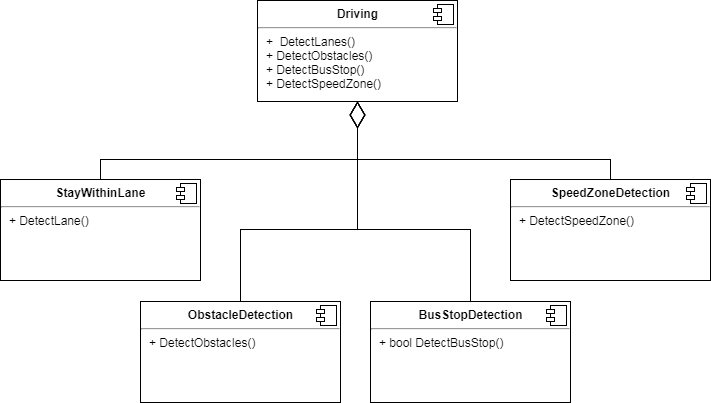
\includegraphics[width=\textwidth]{Images/Design/componentDiagram.png}
    \caption{Major components of functionality in the product; each component deals only with its own concerns}
    \label{fig:components}
\end{figure}
%Jeg er ikke overbevist om at ovenstående diagram er vildt vigtigt når vi nu alligevel har det nedenstående, dog giver det fint mening indtil videre

Note that the components refer not only to software, but also the physical design of the car. For instance, after we implement the driving component in software, we require a functioning LEGO-bus to test the software on. Only after this is done can we conclude whether the component works properly. Reason being that although the software logic might work as intended, incorrect sensor measurements, track/lane inconsistencies and similar need to be taken into account during programming, because otherwise, the product might not work as expected.

\subsection{Assumptions and Guarantees}
For now, we are imagining each component as a black box. What it contains is not of importance, only what it can do. Each component guarantees specific functionality as long as certain assumptions are met, see figure \ref{fig:assumptionGuarantee}. 

\begin{figure}[ht]
    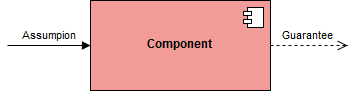
\includegraphics[width=\textwidth]{Images/assumptionGuarantee.png}
    \caption{The assumption-guarantee model}
    \label{fig:assumptionGuarantee}
\end{figure}

Most of the assumptions are made for the sake of simplicity in order to not delude the design with unnecessary detail. In this section, we will specify assumptions and guarantees that are not immediately obvious. Other, common assumptions, like the fact that the bus needs gravity to drive properly, will also still be left implicit. The specifications will later be used for informing the creation of interfaces for the classes of the program. 

We will now further describe the major components in text.
\begin{description}
    %\item[Driving]
    
    \item[Obstacle Avoidance]
    We assume the obstacle is large and made out of material that can be detected consistently by the ultrasonic sensor. 
    
    \item[Stay Within Lane]
    The component assumes perfectly consistent road markings with no imperfections and unintentional holes. 
    
    \item[Cruise Control]
    We assume that the vehicle to follow drives at a speed that makes sense, e.g. not too slow to detect and not too quick to follow. 
    
    \item[Speed Zone Control]
    We assume that each different speed limit is marked with a single sign to be recognized by the nxtCam sensor. 
    
    \item[Manoeuvre]
    We assume that at any point where lane switching is allowed, lines will be replaced with dotted lines. 
    
    The component guarantees that it can park parallel to a bus stop with a maximum distance of 1 cm to the edge at any point. 

    \item[Stop Button]
    Although this fits less well with the reality, we will not be using a physical stop button inside the bus, because this will be tough to click. For this reason, the component assumes that it receives a Bluetooth signal, and will then ensure that the bus halts at the next stop.  
    
    \item[Detect Bus Stop]
    While there are many different types of bus stops, in reality, we assume that there is only a single bus stop design that we need to recognise using the nxtCam sensor. This will be specified during the implementation.
    
    
\end{description}
\section{Software Architecture}

Because we are using nxtOSEK as our operating system for the bus, we can program using either C or C++, see \ref{nxtOSEK} for more details. Because we can split the program cleanly into modular components as shown in the diagram \ref{fig:components}, we will program using the object-oriented programming paradigm in C++. 

Using the separated components as the baseline, we now create a class diagram that is less abstract than the component separation, which we will use as the software architecture of our model (the programming logic of the bus) implementation. Using this diagram, we will later create precise interfaces for all its classes. The dark blue boxes signify the physical sensors that the program will need to communicate with. See figure \ref{fig:softwareArchitecture} 

The arrows on the figure signify function calls, e.g. if an arrow points from object A to B, it means that object A will call functions from object B. To better describe the concerns of each class on the diagram, we've written an example of one function call that might occur between the objects on each edge. This part isn't intended to be extremely precise, however, it helps communicate how we are planning to use object-oriented programming for information hiding and abstraction. See the diagram in figure \ref{fig:softwareArchitecture}

\begin{figure}[ht]
    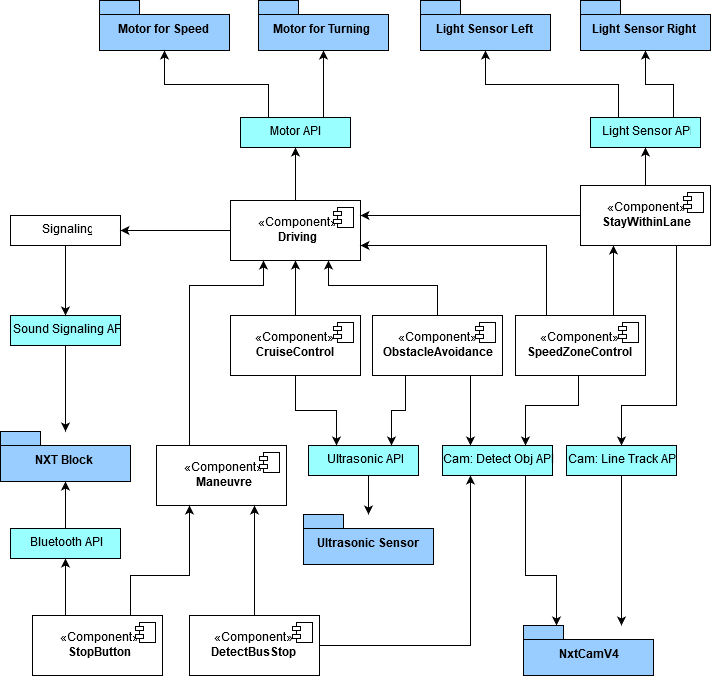
\includegraphics[width=\textwidth]{Images/Design/architectureClassDiagram.png}
    \caption{Class diagram\todo[inline]{From supervisor: This is not a class diagram: class diagram is about inheritance and aggregation, but this one is about how components are connected -- a component diagram?
I still don't understand why you cannot use interface-"arrows":
function is a tiny interface (in general interface may contain multiple functions, but here it seems that one function per interface is enough).} of the program architecture of the model; function call examples are written on the edges.
\todo[inline]{From supervisor: I would still prefer the component diagram notation with bubles and arcs.}
\todo[inline]{From supervisor: I don't understand how this NXT block is connected. It seems to be useless sink of information which does not affect anything.
Is there a remote button somewhere that triggers the StopButton functionality somehow?}}
    \label{fig:softwareArchitecture}
\end{figure}


The intent is that we use this diagram directly for our program architecture so that each object on the diagram becomes a class in the implementation. The light blue coloured API-objects are also classes that we will create ourselves. The point with these is that they expose the useful functions that each sensor/actuator has, while also automatically filtering out incorrect measurements and calibrating the sensors.

Do, however, note that the diagram is still a bit of a simplification. Specifically, the sensor API classes do not communicate directly with their corresponding sensors; instead, they all query the NXT block, that gives access to different functions dependant on which sensors are connected.\todo{From supervisor: Perhaps you can draw a box around APIs to show that they are inside NXT block?} The diagram simply shows the model of the program, so we don't wish to directly deal with these sorts of implementation and low-level details. 

Something to note, which is not mentioned on the diagram, is that we have also planned to write a program separate from the system, which has the one job of sending messages via Bluetooth to the NXT-block whenever we wish to illustrate that a passenger has clicked the stop-button. This is intended to work just like a stub-function would, and the rest of the program simply pretends that a real passenger clicked a button inside the bus.

\section{System Architecture}

\todo{Physical Architectural View}

As previously mentioned, there are many layers of abstraction in the program before one actually reaches the hardware level of the sensors. In this section, we will describe these layers, going from the high-level programming of the model, e.g. the architecture described in figure \ref{fig:softwareArchitecture}, down to the hardware specifics of the sensors themselves. 

The intent is, of course, that these software abstractions will not affect our model implementation, aside from the fact that we have to include some libraries to facilitate sensor communication (for instance "ecrobot\_interface.h" and similar). See figure \ref{fig:abstractionLayers} for the system architecture and its layers of abstraction. The dark blue object "Components" consists of all the software inside the components planned in the previous section \ref{fig:softwareArchitecture}. 

\todo{mention that it is a layer diagram, going from top, high-level to hardware sensors and actuators}
\todo{More corrections from 8/11-2017}
\begin{figure}[H]
    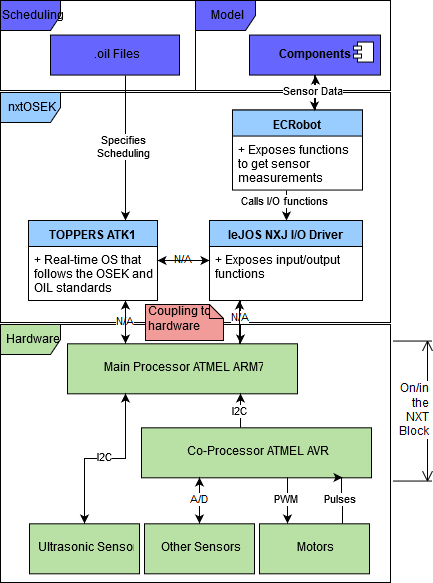
\includegraphics[width=\textwidth]{Images/Design/abstractionLayerDiagram.png}
    \caption{Layer diagram of the system architecture of the product, going from high-level programming down to low-level hardware specifics.
    \todo[inline]{From supervisor: These arrows mean different things than other arrows inside the box, so they must be drawn somehow differently.
I am reading these as layers in OSI model, e.g.
http://www.flickriver.com/photos/phploveme/2911722148/}}
    \label{fig:abstractionLayers}
\end{figure}

The note "Coupling to hardware" and the "N/A" edges exists because those are implementation details inside nxtOSEK, which we do not really have access to\todo{From supervisor: Just treat it as a different abstraction layer. It is not realy an API, nor protocol, but something that "runs on top".}. In the hardware frame, the edges signify communication protocols such as PWM (pulse width modulation, as described in section \ref{analysisMotors}). 

\section{Class Structure and Scheduling}

Previously we broke down the requirements for the functionality of the bus into a number of components, and created a class diagram \todo{Can I call it a class diagram? Call it something else if I change it.}\todo{Missing ref to the class diagram} to structure how those would interact. The next step is to create interfaces and thereby clear, concrete contracts of the intended functionality of each major class in the program. 

In non real-time systems the class and system structure may be enough to start creating interfaces, but in this case we still need to figure out we will reconcile the class structure with the chosen scheduling method. As mentioned in \ref{analysis:scheduling}, we will be using fixed priority scheduling\todo{With or without preemption?} to decide when the tasks in the bus are run. 

One of the questions that we need to clear up is where we run the program from and where the main function resides. Where do we initialise our components and ensure that they deliver their data to the correct receiver? Besides answering these questions, we must ensure that conventions of good object-oriented design are still followed. Specifically, the trouble is keeping a low coupling between the components, even though they all need to communicate with the driving-component. 

\subsubsection{Program Flow}
The program flow and main function is defined within the .oil-files; see a description of these in section \ref{OILteo}. Inside the .oil-files we define functions as tasks which will be called with specific priorities, periods and deadlines. 

The \code{ObstacleDetection}-component (which uses the ultrasonic sensor to check for obstacles ahead of the vehicle) will be used as an example to illustrate the issue. If the program did not have to be a real-time system, then the obvious solution would simply be to detect obstacles regularly. If any are found, then the Driving-component is immediately alerted, which then calls the motor controls and adjust the direction of the bus.

The issue in this case is that the bus might miss a lot of other deadlines while the Driving-component has control of the CPU. This is of course unacceptable, because, depending on the circumstances, the bus might no longer meet its other requirements. 

Imagine the following worst case. The bus detects a bus stop and decides to park there. Now the driving component gains control of the CPU for the next two seconds while it parks the bus. All deadlines are lost in that time, and if there's an obstruction on the road that was not detected prior, it might not be detected until it is too late.\todo{Use a tool to figure this out. Can't think of every situation manually.}

The solution to this is splitting the above task into separate, smaller tasks: sensor detection and the execution of driving commands. Both of these are then be scheduled and executed entirely independently. This means that the system might wait longer before executing a stop-command. However, this should not be a problem, as long as we ensure that the period is short enough, so that the bus can always stop in time before crashing into something. 

This works by having the .oil-files call the individual components as often as necessary, which then return their suggested steering response (continue driving, brake, turn left, etc.) to the Driving-component. The driving component is then called at a separate time to decide which command to execute and do so.

Additionally, this contains the coupling of the program entirely inside the Driving-component and .oil-files. The Driving-component now handles everything in regards to input and output of the different components, and also deals with prioritising the steering commands, to figure out what the motor should actually do if there is any ambiguity (imagine it both found a bus stop and an obstruction in the road). 

Imagine a case where the scheduler first selects the \code{ObstacleDetection}-component to control the CPU, and an obstacle is detected, and the car is stopped. See the sequence diagram in figure \ref{fig:sequenceDetectObstacle} for how the program flow would look.

\begin{figure}[ht]
    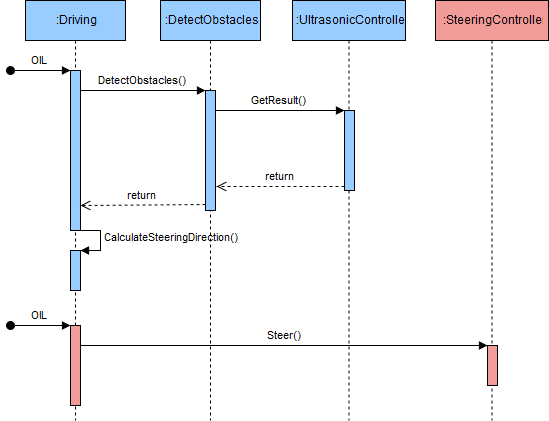
\includegraphics[width=\textwidth]{Images/Design/sequenceObstacleDetection.png}
    \caption{Sequence diagram showing the program flow while detecting obstacles and reacting to this.}
    \label{fig:sequenceDetectObstacle}
\end{figure}

s\todo{From supervisor: This communication can be through shared variable(s): e.g. obstacle detector is being run periodically and then marks some variables that there is some obstacle somewhere, then the driver could be running at its own pace and check the obstable variables.
It is not clear how/why do you actually structure/map classes to tasks and how/why things are connected.
In this picture it is clear that communication between classes are synchronous function/method calls, but it does not neccessarily have to be this way.
It seems that you are not exploiting (pseudo)parallelism and your tasks seem sequential (one after another).}

Task A calls the \code{ObstacleDetection}-component, which then returns results from the ultrasonic sensor. The priority of all currently saved steering-commands is then calculated and saved locally in the Driving-component. At this point the control is returned to the .oil file. 

Then task B assigns control of the CPU to the driving component a second time, which executes the highest priority steering command, which in this case is to brake the car\todo{Couldn't this be done with a quick command instead? "motor speed = 0", no need to have the driving component to do this.}. Task B is fully separate from obstacle detection, and regardless of which task was executed prior, task B just executes the top priority command. 

%The question is where our individual program flows are called. We have a few options, none of which seem immediately better than the rest:
%- Each component is called on its own. This makes it so the .oil programmer needs to know about the functions of all the different class functions (and where to initialize a call). This can be remedied with an interface that exposes a .Run() method. Problem here is what to do with the result of each call. If the Obstacle Detection class decides that the bus should now stop, what does it do? Does it have access to the Driving component and can it call the .Brake() function? But then all functions have access to the Driving component, which heavily increases the coupling of the program (not good). Does it expose its return value as an event that is subscribed to by the Driving component? But then the worst case execution time becomes difficult to control, because unless we know the entire program, we cannot say how many items are subscribed. Does it expose its value as a property? But then, all classes need to expose a property of the same type and also use it in the same way. Again, this increases the coupling of the program. 



\todo{Add one line descriptions of the scope (intended functionality) of the different classes. Add it into the class diagram perhaps. For instance: Maneouvre-component "high-level driving commands".Remove maneuvre from all this shit}

%Driving has RequestSequenceOfCommands(list<enum DrivingCommand>, enum sender)
%drivingCommand cannot be enum, because it needs parameters, so just a class

%The solution we chose:
%One task for each component, with differing periods and deadlines.
%One task for controlling the motors.

%These tasks are all initialized from the Driving-component. So in the case where we check for obstacles, see the following sequence diagram:
%1. Oil -> Driving.DetectObstacles() -> DetectObstacles:GetResult() -> UltrasonicController.GetResult() -return to detectObstacles-> Driving.SetPriority() -return to Oil->
%2. Oil -> Driving.Steer() -> SteeringController.Steer(Command) -> MotorForSteering -return to steeringController-> MotorForSpeed

%Task 1 detects whether there are any obstacles on the track and places the suggested response (probably braking) at the top of the priority queue. 


\todo{Oprems ALLE tasks. Skriv også om vores TaskMain, som har prioritet på 0, men startes først, og har en uendelig while løkke hvor programmet busy-waiter hvis ikke det ellers kører andre tasks. Kunne man have gjort det på en anden måde? }
\section{Interfaces}
In this section, we specify interfaces for all objects in the software model, as seen in figure \ref{fig:softwareArchitecture}. This includes the sensor controllers, which are intended to abstract from hardware specific information like the calibration of sensors and filtering out incorrect measurements from the raw data. 

\subsection{Sensor Controllers}
The sensor controller classes all require a calibrate-method, which is called whenever the bus starts, in order to ensure the sensors and motors work as intended. Inheritance is utilised to show this similarity between the individual Sensor Controllers. See figure \ref{fig:interfaceSensorControllers} for a class diagram showing the hierarchy, functions and properties of the Sensor Controllers. Note that constructors and destructors are omitted from this, as they provide little insight to the functionality of the classes. 

\subsection{SensorControllers}
See figure \ref{fig:interfaceSensorControllers} 

\begin{figure}[ht]
    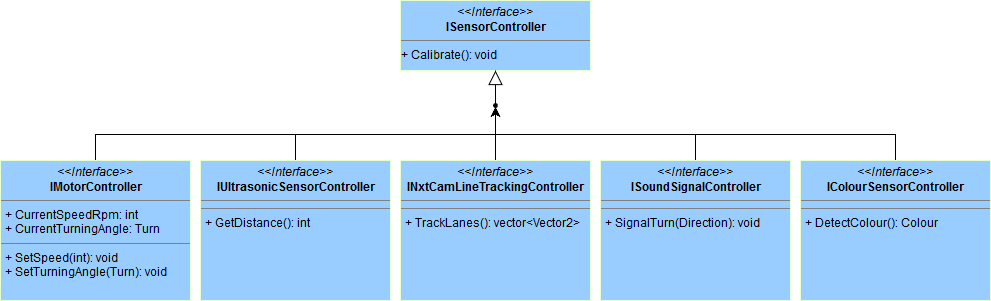
\includegraphics[width=\textwidth]{Images/Design/InterfaceSensorControllers.png}
    \caption{Class diagram showing the sensor controller interfaces}
    \label{fig:interfaceSensorControllers}
\end{figure}

\code{Turn} is a class containing the degrees and direction of the specified turn that is to be executed. \code{Direction} and \code{Colour} are both enumeration types that contain a number of associated options (e.g. left or right, or different colours). Rpm from \code{CurrentSpeedRpm} abbreviates rotations per minute.

\subsection{Components}
The components call the sensor controllers in order to obtain the necessary sensor measurements, and also call the calibration of their corresponding sensors. See figure \ref{fig:interfaceComponents} for a class diagram describing the planned interface structure.

\begin{figure}[ht]
    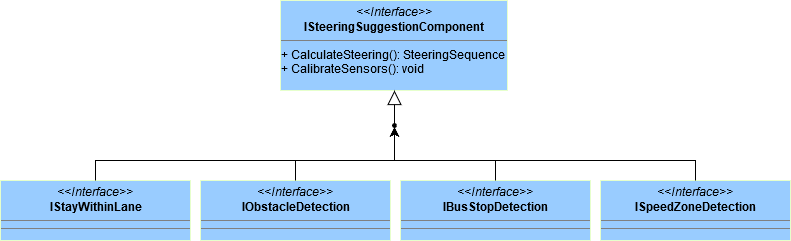
\includegraphics[width=\textwidth]{Images/Design/InterfaceComponents.png}
    \caption{Class diagram showing the component interfaces}
    \label{fig:interfaceComponents}
\end{figure}

All components have their \code{CalculateSteering}-method called by the \code{Driving}-component, to which they then return the \code{SteeringSequence} that they suggest the bus should drive. Based on the values it gets, the \code{Driving}-component later decides how to actually drive. 

The class \code{SteeringSequence} contains one or multiple \code{SteeringCommands}, which contains a distance, speed and a \code{Turn} that the bus should drive. Multiple \code{SteeringCommands} can be used for things like braking the bus smoothly through multiple steps, or stopping at a bus stop and other similar manoeuvres. 



\todo{This has changed, so change the diagram: remove the ISteeringSuggestionComponent superclass, remove calibration and add the different return values below. Similarly, the entirety of the design chapter has a few outdated diagrams, which need to be fixed.}

%Right now it's planned the following way: Every time we start executing a new command we note how much distance that command wants to cover (fx. drive 50km/hr for 30 meters). Then, every time steer is called, we start a new command only if the current command is finished. If the SteeringSequence is still at the top of the queue, we move on with the next command in the sequence, and if it's not then we do the other SteeringCommand, then later we continue the Sequence.

%Maybe we need to give the components information about what they signalled last time? They should keep that info themselves, if necessary. 

\subsection{Driving}
\code{Driving} is the class that couples the system. As such, it initialises the classes (calibrating the sensors at the same time), calls the components and decides how to steer the bus. See figure \ref{fig:interfaceDriving} for the interface of the \code{Driving} class.

\begin{figure}[ht]
    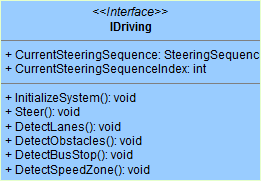
\includegraphics[]{Images/Design/interfaceDriving.png}
    \caption{Interface of the driving class}
    \label{fig:interfaceDriving}
\end{figure}



\todo{Write the following comment in english to cap off the section:}
%I programmet bruger vi ikke rent faktiske interfaces af to grunde. Først og fremmest programmerer vi i C++, der ikke giver elegant understøttelse af interfaces. Derudover laver vi et realtidssystem, og da der ikke direkte er noget krav for klar modularitet og udskiftelige komponenter, så er det så at sige en unødvendig brug af den begrænsede hukommelse vi har på Nxt'en.

Additional to the software and system architecture, we will also design the bus itself along with the track that it needs to drive on. 
\todo{Write about the OSEK standard, And thereby also OIL, However, probably not in this chapter}

\section{Design of the track}\label{trackDesign}

In order to validate that the requirements of the project are met. A track for the bus which is designed based on the requirements had to be made. This section will detail the design decisions made when designing this track. 

%Firstly the setup
First, let us start with a short reminder: The track should have two lanes, as to mimic the pre-existing infrastructure, which usually has bidirectional roads. Furthermore, the track should have bus stops that the vehicle can drive into, such that passengers can get on/off the bus. The bus stops need to have a minimum length equivalent to the length of the bus in addition to the space that is needed to drive into and out of the bus stops.

Based on this the we know that the track should have proportions based on the scale of the bus. Also we know that the track should include turns as sharp as in real life\cite{DriveingCurves}. The width of the road should also be designed after real danish roads based on the laws given by the Danish road directorate \cite{roadRules}.  As such the track needs to be designed such that the bus has the needed space to turn smoothly.

To help the sensors detect when to switch to a bus stop lane, the track should have special coloured tape placed a specified distance away from the bus stops, which sensor(s) can recognise.

To draw the track that the bus will drive on, black tape is used such that the sensors, which perform line tracking can detect the lines. The sensors are more effective at detection when working with colours with strong contrast, therefore we chose black and white. Black tape and white backdrop have been chosen over white tape and black backdrop. White lines and black backdrop are more true to life, but the results are the same, so since a white backdrop was more accessible, this was chosen.

Bus stops can in principle come in many forms, however, we will focus on a single bus stop design. This design must have enough space

The following is a brief explanation of the relevant rules that real life roads must follow and therefore our track has to follow. There are of course allot of rules, that are irrelevant for this project, e.g. the thickness of a road. 

%Calculated based on the danish road directorate, see "Calculation of maximal turn angle of a bus road" in appendix \ref{laneCalculations}, if a 12 meter bus can drive on a road with with a front wheel turn angle of 28.6 with a 0.3 meter leeway to each side at 15 km/t\cite{DriveingCurves}. this is the simple turn where the bus has no room to perform a small turn to the opposite direction to make a sharper turn, see\cite{DriveingCurves} for a illustration of the manoeuvre.

The minimal width of the road, set forth by the road directorate, is not constant. On a straight or mildly curving road, the standard width of the road is 3.5 meters. However, when the road has a sharp turn the road other rules apply. 

Let us start with the rules for straight roads as previously stated a bus road in the city has to be 3.5 meters wide\cite{roadRules}. 3 meters is allowed on short straight stretches, however, this is not the standard so this number is discarded for now. We also know from the Danish road directorate that the maximum width of the bus is 2.55 meters\cite{DriveingCurves}. From this the proportions are calculated, see 1 in appendix \ref{laneCalculations} for the specific calculations.

For the curved roads, the Danish road directorate has set forth a number of conditions for the approval of roads and the vehicles that are allowed to use the road. In order for a bus of 12 meters in length to be allowed to drive on a road, the road has to abide by the following condition.
A bus 12 meters in length, must be able to pass through the road with a front wheel turning angle of maximum  28.6 degrees, see 2.1 in appendix \ref{laneCalculations}, while keeping 0.3 meters leeway to each side at any point\cite{DriveingCurves}, or it must have an area to be able to turn a bit to the opposing side, so that it can make a sharper turn. However, we have chosen to refer to the simple turn as our requirement. According to these requirements, the calculations found in section 2 appendix \ref{laneCalculations} were made, to ensure that the track conforms to this rule.
The length of the bus stop has been found by finding the minimum distance that the bus needs to drive into and out of the bus lane, and then added to the length of the bus. The formula can be seen in \cite{busstoplength} and comes out to ~56.4. However, this would require the bus to enter the bus stop at a very steep angle that will not be possible at most roads, so a big amount of additional space has been added to the bus stop.

According to these rules, the following design in Figure \ref{fig:TrackDesign} was made. The image is not to scale and its given in cm.

\begin{figure}[ht]
    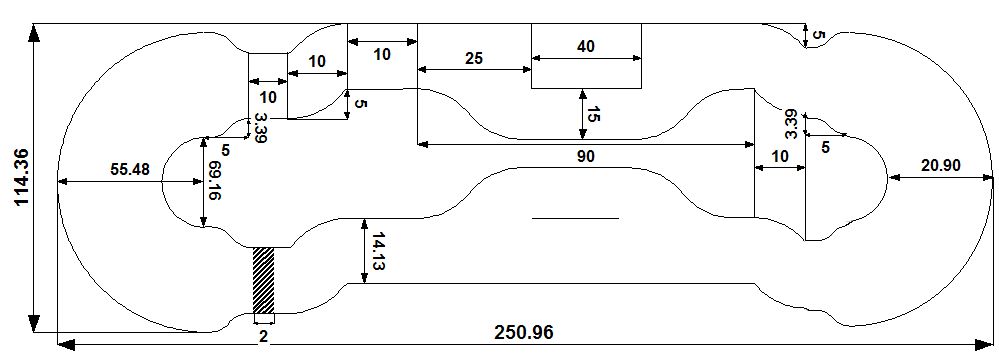
\includegraphics[width=1\textwidth]{Images/Design/TrackDesign.PNG}
    \caption{Track design}
    \label{fig:TrackDesign}
\end{figure}






%Straight bus lane calculations -1
%Calculation of maximal turn angle of a bus road -2.1
%From straight to turning width calculations -3
%Turning bus lane radius calculation -2


%beskriv bus stop: 45 grader ind, 45 grader ud, bus bredde + 2 cm, bus længde 
%der er mange forskellige busstoppesteder, så vi vælger bare et design



% Selected Sensors:
%     \item[(4) Detecting Obstacles]
%    We intend to detect obstacles using a single sensor, which turns on whenever the bus is instructed to switch lanes, as to verify that no obstacles are found in the other lane. If this does not work, multiple sensors may be needed.